\documentclass[12pt, a4paper]{article}

% ── Packages ───────────────────────────────────────────────────
\usepackage[utf8]{inputenc}
\usepackage[T1]{fontenc}
\usepackage{geometry}
\geometry{margin=2.5cm}
\usepackage{graphicx}
\usepackage{amsmath, amssymb}
\usepackage{booktabs}
\usepackage{hyperref}
\usepackage{listings}
\usepackage{xcolor}
\usepackage{tikz}
\usetikzlibrary{shapes.geometric, arrows.meta, positioning, fit}
\usepackage{float}
\usepackage{enumitem}
\usepackage{caption}

\lstset{
  basicstyle=\ttfamily\small,
  keywordstyle=\color{blue},
  commentstyle=\color{gray},
  stringstyle=\color{red},
  breaklines=true,
  frame=single,
  numbers=left,
  numberstyle=\tiny\color{gray},
}

\title{%
  \textbf{Mixture-of-Experts Framework for Mid-Price Movement Prediction} \\[0.5em]
  \large Implementation Report — FI-2010 Benchmark Dataset
}
\author{Group XX — B.Tech 4th Year}
\date{\today}

% ═══════════════════════════════════════════════════════════════
\begin{document}
\maketitle
\tableofcontents
\newpage

% ── 1. INTRODUCTION ───────────────────────────────────────────
\section{Introduction}

This report documents the design, implementation, and evaluation of a \textbf{Mixture-of-Experts (MoE)} framework for predicting short-term mid-price movements from high-frequency limit order book (LOB) data. The system is built on the \textbf{FI-2010 benchmark dataset} and addresses a 3-class classification problem: Up, Stationary, or Down movement at prediction horizon $k=10$.

The project extends beyond pure classification by incorporating:
\begin{itemize}
  \item A \textbf{signal-based strategy layer} that converts probabilistic predictions into Buy/Hold/Sell/Flat trading signals.
  \item A \textbf{backtracking module} for online adaptation of expert weights and strategy thresholds.
  \item A \textbf{backtesting engine} that simulates portfolio performance with realistic transaction costs.
\end{itemize}

\subsection{Constraints}
\begin{itemize}
  \item No deep learning architectures (CNNs, LSTMs, Transformers) — only classical ML models.
  \item Feature engineering is limited to basic LOB-derived features already present in FI-2010.
  \item No forward-looking bias at any stage of the pipeline.
\end{itemize}

% ── 2. DATASET ────────────────────────────────────────────────
\section{Dataset: FI-2010}

\subsection{Overview}
The FI-2010 dataset~\cite{ntakaris2020} provides normalised limit order book snapshots from five Finnish stocks traded on NASDAQ Nordic. Each sample contains \textbf{144 features} derived from the 10-level LOB and \textbf{labels at five prediction horizons} ($k \in \{1, 2, 3, 5, 10\}$).

\subsection{Feature Structure (144 features)}
\begin{itemize}
  \item \textbf{Features 0–39}: Level-1 to Level-10 raw LOB (ask price, ask volume, bid price, bid volume) — $10 \times 4 = 40$ features.
  \item \textbf{Features 40–79}: Time-insensitive features (spread, mid-price, price differences, mean prices/volumes at multiple depth levels).
  \item \textbf{Features 80–119}: Time-sensitive features (relative price changes, intensity of price movements).
  \item \textbf{Features 120–143}: Deep statistical features (accumulated differences, order-flow imbalance over windows).
\end{itemize}

\subsection{Labels}
\[
y_t = \begin{cases}
  0 & \text{(Up)}  \quad\quad\text{if } m_{t+k} > m_t + \epsilon \\
  1 & \text{(Stationary)} \quad\text{if } |m_{t+k} - m_t| \leq \epsilon \\
  2 & \text{(Down)} \quad\;\text{if } m_{t+k} < m_t - \epsilon
\end{cases}
\]
where $m_t$ is the mid-price and $\epsilon$ is a smoothed threshold.

\subsection{Cross-Validation: Anchored Forward Walk}
The dataset ships with 9 pre-split folds. Training data grows cumulatively (anchored) while the test set is the next unseen trading day. This prevents \textbf{temporal leakage} — a critical requirement for financial time-series.

\subsection{Class Imbalance}
The \textit{Stationary} class dominates ($\sim$40\% of samples). We use \textbf{balanced class weights} computed via scikit-learn's \texttt{compute\_class\_weight('balanced')} to compensate.

% ── 3. PIPELINE OVERVIEW ─────────────────────────────────────
\section{Pipeline Overview}

The full pipeline has five stages executed per fold:

\begin{figure}[H]
\centering
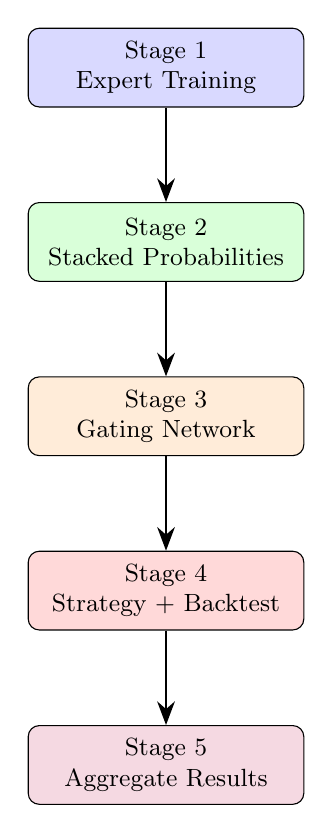
\begin{tikzpicture}[
  block/.style={rectangle, draw, rounded corners, minimum width=3.5cm,
                minimum height=1.0cm, align=center, font=\small},
  arr/.style={-{Stealth[length=3mm]}, thick},
  node distance=1.2cm
]
  \node[block, fill=blue!15]  (s1) {Stage 1\\Expert Training};
  \node[block, fill=green!15, below=of s1] (s2) {Stage 2\\Stacked Probabilities};
  \node[block, fill=orange!15, below=of s2] (s3) {Stage 3\\Gating Network};
  \node[block, fill=red!15, below=of s3] (s4) {Stage 4\\Strategy + Backtest};
  \node[block, fill=purple!15, below=of s4] (s5) {Stage 5\\Aggregate Results};

  \draw[arr] (s1) -- (s2);
  \draw[arr] (s2) -- (s3);
  \draw[arr] (s3) -- (s4);
  \draw[arr] (s4) -- (s5);
\end{tikzpicture}
\caption{Pipeline stages executed per cross-validation fold.}
\end{figure}

% ── 4. STAGE 1: EXPERT MODELS ────────────────────────────────
\section{Stage 1: Expert Models}

Three heterogeneous classifiers form the expert pool:

\subsection{Expert 1: Logistic Regression (LR)}
\begin{itemize}
  \item \textbf{Model}: Multinomial LR with L2 regularisation.
  \item \textbf{Hyperparameter tuning}: $C \in \{0.001, 0.01, 0.1, 1.0, 10.0\}$ via 3-fold stratified CV, optimising macro-F1.
  \item \textbf{Calibration}: Post-hoc \textbf{isotonic regression} via \texttt{CalibratedClassifierCV}.
  \item \textbf{Role in MoE}: Captures linear decision boundaries. Fast to train, provides a stable baseline.
\end{itemize}

\subsection{Expert 2: XGBoost}
\begin{itemize}
  \item \textbf{Model}: Gradient-boosted trees with softmax objective.
  \item \textbf{Hyperparameters}: max\_depth $\in \{3,4,5,6\}$, learning\_rate $\in \{0.01, 0.05, 0.1\}$, up to 800 trees with \textbf{early stopping}.
  \item \textbf{Regularisation}: $\alpha = 0.1$ (L1), $\lambda = 1.0$ (L2), min\_child\_weight = 3.
  \item \textbf{GPU acceleration}: Uses \texttt{gpu\_hist} tree method when CUDA is available.
  \item \textbf{Calibration}: Isotonic regression.
  \item \textbf{Role in MoE}: Captures non-linear feature interactions, handles feature heterogeneity.
\end{itemize}

\subsection{Expert 3: Multi-Layer Perceptron (MLP)}
\begin{itemize}
  \item \textbf{Architecture}: Input($144 \times 5$) $\to$ Dense(256, BN, ReLU, Drop=0.3) $\to$ Dense(128, BN, ReLU, Drop=0.3) $\to$ Dense(3).
  \item \textbf{Temporal framing}: Stacks 5 consecutive time steps (lookback=5), giving $144 \times 5 = 720$ input features.
  \item \textbf{Loss}: Focal Loss ($\gamma=2.0$) with balanced class weights — down-weights easy examples.
  \item \textbf{Optimiser}: Adam ($lr=10^{-3}$, weight\_decay=$10^{-5}$).
  \item \textbf{Scheduler}: ReduceLROnPlateau (factor=0.5, patience=3).
  \item \textbf{Stability}: Gradient clipping (max\_norm=1.0).
  \item \textbf{Calibration}: Learnable temperature scaling parameter.
  \item \textbf{Role in MoE}: Captures temporal patterns across consecutive LOB snapshots.
\end{itemize}

\subsection{Why These Three Experts?}
\begin{enumerate}
  \item \textbf{Diversity}: LR (linear), XGBoost (tree-based), MLP (neural) — maximally diverse model families ensure complementary error patterns.
  \item \textbf{Computational feasibility}: All train in minutes on a single GPU.
  \item \textbf{Interpretability}: LR coefficients are interpretable; XGBoost provides feature importance; MLP captures interactions.
\end{enumerate}

% ── 5. STAGE 2: STACKED PROBABILITIES ────────────────────────
\section{Stage 2: Stacked Probability Generation}

To train the gating network without overfitting to the training labels, we use \textbf{3-fold inner cross-validation} (stacking):

\begin{enumerate}
  \item Split training data into 3 stratified inner folds.
  \item For each inner fold: train fresh LR, XGB, MLP on the inner training split.
  \item Predict \textit{out-of-fold} probabilities on the held-out inner validation split.
  \item Concatenate to form $\mathbf{P}^{\text{stacked}} \in \mathbb{R}^{N_{\text{train}} \times 9}$.
\end{enumerate}

\textbf{Key detail}: Inner MLP training uses \texttt{verbose=False} to prevent console output interleaving.

% ── 6. STAGE 3: GATING NETWORK ───────────────────────────────
\section{Stage 3: Gating Network}

\subsection{Architecture}
\[
\text{Input}(12) \xrightarrow{} \text{Dense}(64, \text{ReLU}, \text{Dropout}=0.2) \xrightarrow{} \text{Dense}(3, \text{Softmax})
\]

\textbf{Input (12-dimensional)}:
\begin{itemize}
  \item 9 dimensions: concatenated expert probabilities $[\mathbf{p}_{\text{LR}}, \mathbf{p}_{\text{XGB}}, \mathbf{p}_{\text{MLP}}]$.
  \item 3 dimensions: \textbf{expert agreement features} — for each class $c$, the standard deviation of $\{P_{\text{LR}}(c), P_{\text{XGB}}(c), P_{\text{MLP}}(c)\}$.
\end{itemize}

High agreement std means experts disagree on class $c$ — the gating network can learn to be cautious in such cases.

\subsection{Training}
\begin{itemize}
  \item \textbf{Loss}: NLLLoss on the weighted combination $P_{\text{final}} = \sum_i w_i \cdot P_i$.
  \item \textbf{Optimiser}: Adam ($lr = 10^{-3}$, weight\_decay = $10^{-4}$).
  \item \textbf{Early stopping}: Patience = 8 epochs on a 15\% validation split.
\end{itemize}

\subsection{MoE Forward Pass}
\[
P_{\text{final}}(c) = w_1 \cdot P_{\text{LR}}(c) + w_2 \cdot P_{\text{XGB}}(c) + w_3 \cdot P_{\text{MLP}}(c)
\]
where $\mathbf{w} = g(\mathbf{p}^{\text{stacked}})$ is the softmax output of the gating network.

% ── 7. STAGE 4: STRATEGY + BACKTEST ──────────────────────────
\section{Stage 4: Strategy Layer, Backtracking, and Backtesting}

\subsection{Strategy Layer}

Converts the probability vector into a trading action using a \textbf{signal-based state machine}:

\[
\text{signal}_t = P(Up)_t - P(Down)_t
\]

\begin{enumerate}
  \item \textbf{EMA smoothing}: $s_t^{\text{ema}} = \alpha \cdot s_t + (1-\alpha) \cdot s_{t-1}^{\text{ema}}$ with $\alpha=0.3$ — reduces noisy oscillations.
  \item \textbf{Entry}: If $|s^{\text{ema}}| > \tau_{\text{entry}} = 0.35$ and directional $P > \theta = 0.55$ and regime filter is valid $\to$ Buy or Sell.
  \item \textbf{Exit}: If $|s^{\text{ema}}| < \tau_{\text{exit}} = 0.10$ and currently in position $\to$ Flat.
  \item \textbf{Flip penalty}: Reversals (Long$\to$Short or vice versa) require extra signal strength ($+0.10$).
  \item \textbf{Regime filter}: Average of max(P(Up), P(Down)) over last 10 steps must exceed 0.45.
\end{enumerate}

\subsection{Multi-Horizon Agreement Filter}

Before executing a Buy/Sell, we check whether the k=5 directional prediction (from the LR expert) agrees with the k=10 MoE prediction. Disagreement downgrades the action to Hold.

\subsection{Backtracking Module}

An \textbf{online adaptive module} that operates during inference:

\begin{itemize}
  \item \textbf{Buffer}: Rolling window of 200 recent (prediction, action, outcome) tuples.
  \item \textbf{Update}: Every 100 steps, computes per-expert accuracy and adjusts:
  \begin{enumerate}
    \item Expert weights via exponential update: $w'_i \propto w_i \cdot \exp(\eta \cdot \alpha_i^{\text{EMA}})$
    \item Strategy thresholds $\theta_{\text{buy}}, \theta_{\text{sell}}$ based on FP/FN rates.
  \end{enumerate}
  \item \textbf{Weight clamping}: $w_i \in [0.10, 0.60]$ — prevents degenerate weighting.
  \item \textbf{Action correction}: If signal strongly contradicts previous action, override to Hold.
\end{itemize}

\subsection{Backtesting Engine}

Simulates a trading portfolio:

\begin{itemize}
  \item \textbf{Positions}: Long, Short, or Flat.
  \item \textbf{Transaction costs}: $c_{\text{total}} = c_{\text{commission}} + c_{\text{spread}} = 0.0001 + 0.0001 = 0.02\%$ per side.
  \item \textbf{Minimum hold}: 15 ticks — prevents over-trading.
  \item \textbf{Returns}:
  \begin{itemize}
    \item Long: $r_t = \frac{m_{t+1} - m_t}{m_t}$
    \item Short: $r_t = -\frac{m_{t+1} - m_t}{m_t}$
  \end{itemize}
\end{itemize}

% ── 8. METRICS ────────────────────────────────────────────────
\section{Evaluation Metrics}

\subsection{Classification Metrics}
\begin{itemize}
  \item \textbf{Accuracy}: Overall fraction of correct predictions.
  \item \textbf{Macro-F1}: Unweighted average of per-class F1 scores — handles class imbalance.
  \item \textbf{Per-class F1}: Individual F1 for Up, Stationary, Down.
\end{itemize}

\subsection{Financial Metrics}
\begin{itemize}
  \item \textbf{Cumulative Return}: $(V_T - V_0) / V_0$
  \item \textbf{Sharpe Ratio}: $\frac{\mu_r}{\sigma_r} \cdot \sqrt{N_{\text{ann}}}$ where $N_{\text{ann}} = 252 \times 390$ (annualised for intraday data)
  \item \textbf{Max Drawdown}: $\max_t \frac{\text{peak}_t - V_t}{\text{peak}_t}$
  \item \textbf{Win Rate}: Fraction of profitable completed trades.
  \item \textbf{Decision Accuracy}: Fraction of Buy/Sell actions that match the true direction.
  \item \textbf{Profit Factor}: Gross Profit / Gross Loss.
  \item \textbf{Turnover}: Fraction of steps with trade actions.
\end{itemize}

% ── 9. AVOIDING FORWARD-LOOKING BIAS ─────────────────────────
\section{Avoiding Forward-Looking Bias}

Several design choices prevent information from the future leaking into predictions:

\begin{enumerate}
  \item \textbf{Anchored forward CV}: Training always precedes test temporally.
  \item \textbf{Inner CV for stacking}: Expert probabilities fed to the gating network are \textit{out-of-fold} — never from the same training samples.
  \item \textbf{Online backtracking}: Weights and thresholds adapt only using past observations in the buffer.
  \item \textbf{Strategy simulation}: The backtesting engine processes samples strictly in order; actions at time $t$ use only information available at time $t$.
  \item \textbf{No future features}: All 144 FI-2010 features are derived from the current and past LOB state.
\end{enumerate}

% ── 10. REFERENCES ────────────────────────────────────────────
\begin{thebibliography}{9}
\bibitem{ntakaris2020}
A. Ntakaris, M. Magris, J. Kanniainen, M. Gabbouj, and A. Iosifidis,
``Benchmark dataset for mid-price forecasting of limit order book data with machine learning methods,''
\textit{Journal of Forecasting}, arXiv:1705.03233v5, 2020.

\bibitem{kercheval2015}
A. N. Kercheval and Y. Zhang,
``Modelling high-frequency limit order book dynamics with support vector machines,''
\textit{Quantitative Finance}, vol.~15, no.~8, 2015.

\bibitem{jacobs1991}
R. A. Jacobs, M. I. Jordan, S. J. Nowlan, and G. E. Hinton,
``Adaptive mixtures of local experts,''
\textit{Neural Computation}, vol.~3, no.~1, pp.~79--87, 1991.
\end{thebibliography}

\end{document}
